\subzag{Экспериментальне исследования $\hbox{\bf g}_{\hbox{\bf 2}}$}
\markright{\hfill\small Экспериментальне исследования $g_2$ \hfill}{}

В настоящее время появилось много теоретических исследований спектрального состава и интегральной интенсивности деполяризованной части рассеянного света (ДРС) (так называемого крыла линии Рэлея --- КЛР). За появление КЛР ответственны флуктуации в ориентациях оптически анизотропных молекул в жидкости и характер их развития во времени.

Многочисленные молекулярные теории позволяют интерпретировать полуширину узкого контура, наблюдаемого в КЛР в жидкостях с анизотропными молекулами как величину, обратную времени релаксации в ориентациях анизотропных молекул механизмом вращательной диффузии.
Полученная таким образом величина $\tau_{\hbox{расс.}}$ характеризует движение 
<<квазичастиц>>, т. е. оказывается чувствительной к образованию ассоциаций, комплексов и, в конечном счете зависит от величины парных ориентационных корреляций $g_2$. 

Для измерения $g_2$ по зависимости интегральной интенсивности ДРС в чистой жидкости от температуры необходимы экспериментальные установки, не выпускаемые промышленностью.
Помимо указанной в рис. 4.4.7 работы по изучению зависимости $g_2$ от плотности в изотропной фазе МББА следует отметить исследование Н.~Б.~Рождественской
и Клауса Эйднера, где были изучены три нематических 
жидких кристалла в изотропной фазе,
отличающиеся величиной и направлением дипольного момента, 
величиной оптической анизотропии и <<жесткостью>> остова молекулы:

4-Этоксибензал-4''-н.-бутиланилин (ЭББА)


\centerline{\hbox{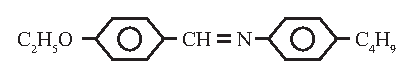
\includegraphics[scale=1]{Ris/ris_eps/ris5exp01.eps}},}

4-н.-Амилокси-4''-н.-амилтолан (ААТ)


\centerline{\hbox{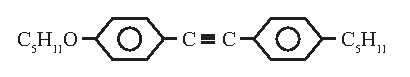
\includegraphics[scale=1]{Ris/ris_eps/ris5exp02.eps}},}

4-н.-Бутилфениловый эфир-4''-н.-гексилоксикарбонилоксибензойной кислота (БГБ)


\centerline{\hbox{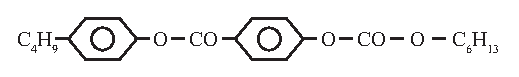
\includegraphics[scale=1]{Ris/ris_eps/ris5exp03.eps}}.}

Полученные результаты представлены на рис. 4.4.8. Для температурной зависимости фактора $g_2$ в изотропном состоянии жидкого кристалла де Женом была выведена следующая формула:
$$ g_2={bT\over (T-T^*)^{\gamma}}, \noq$$
где $T^*$ --- температура несколько ниже ($\sim 1^{\circ}$) точки просветления.
Так как при приближении к высоким температурам $g_2$ должен стремиться к 1, можно ожидать, что в этой формуле $b=1$.


\begin{figure}[tbp]
\centerline{\hbox{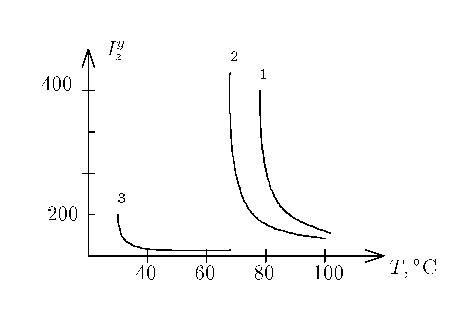
\includegraphics[scale=1]{Ris/ris_eps/ris4_4_08_1.eps}}}

\risp{8}{Температурная зависимость интегральной интенсивности}\centerline{\ris в ЭББА (1), ААТ (2) и БГБ (3)}
\end{figure}

Из графиков на рис. 4.4.8 мы видим, что отклонение от прямолинейной зависимости $(g_2=1)$ наблюдаетя за несколько градусов до резкого возрастания интенсивности, т. е. молекулы с понижением температуры постепенно выстраиваются параллельно направлению <<директора>> (направление, в котором выстраиваются все молекулы, когда интегральная интенсивноть стремится к бесконечности).

Рентгеноструктурный анализ показывает, что в жидкостях вблизи тройной точки существует <<ближний порядок>>, соответствующий взаимному расположению молекул в молекулярном кристалле как в первой, так и во второй координационной сфере.
Исследования температурной зависимости интегральной интенсивности ДРС привели к пониманию существования одновременно нескольких <<локальных структур>>;
доля каждой из них может изменяться в зависимости от температуры жидкости.

Локальная структура может быть определена как стабильная конфигурация расположения молекул и определяется
<<формой>> молекул в жидкости.
В свою очередь форма определяется короткодействующей жесткой отталкивательной частью межмолекулярного потенциала.
Эти отталкивательные взаимодействия --- непрерывные быстроменяющиеся функции положений и ориентаций молекул.

Для исследования структуры и межмолекулярного взаимодействия в жидкой фазе необходимо сочетание диффракционных экспериментов (рассеяние нейтронов, $x$-лучей, деполяризованного рассеяния света) с рассчетами, основанными на статистической механике и термодинамике жидкости.
Для того чтобы успешно использовать численные методы молекулярной динамики
(метод Монте-Карло, интегральное уравнение RISM-модели) для расчета парных корреляционных функций, необходимо выбрать реалистичную функцию парного молекулярного потенциала.
Успешно используются многими авторами функции взаимодействия, полученные квантово-механическим расчетами дисперсионной энергии и отталкивательных членов.
Преобладающие члены в потениале взаимодействия возникают от дисперсионных сил мультиполей между мгновенными электрическими моментами.
Все члены серии мультиполей дают вклад в притяжение: индукционное и диполь-дипольное взаимодействия имеют $r^{-6}$ зависимость, диполь-квадрупольные~--- $r^{-8}$ зависимость, квадруполь-квадрупольные~--- $r^{-10}$ зависимость.

Для молекул с постоянными дипольными моментами эффект коротко-действующего отталкивания, обуславливающего существование локальной структуры, размывается и перекрывается сильными долгодействующими диполь-дипольными взаимодействиями.
Поэтому для изучения проблемы существования локальных структур впервые были
выбраны молекулы без постоянного дипольного момента, но с большим квадрупольным моментом:
$$\hbox{бензол}\hskip 4mm \Theta=-(29,0\pm1,7)\times10^{-40}\hbox{м}^2$$

$$\hbox{гексафторбензол}\hskip 4mm \Theta=+(31,0\pm1,7)\times10^{-40}\hbox{м}^2$$

Экспериментальные исследования были проведены в Санкт-Петербургском государственном университете Н.~Б.~Рождественской и Л.~В.~Смирновой в 1986---1990 годах.
Установка была откалибрована по абсолютным измерениям 3 жидкостей:
CCl$_4$ ($n=\hbox{1,47}$); бензол ($n=\hbox{1,50}$); CS$_2$ ($n=\hbox{1,65}$). 
Температурная зависимость интегральной интенсивности ДРС для бензола представлена на  рис. 4.4.9.

\begin{figure}[tbp]
\centerline{\hbox{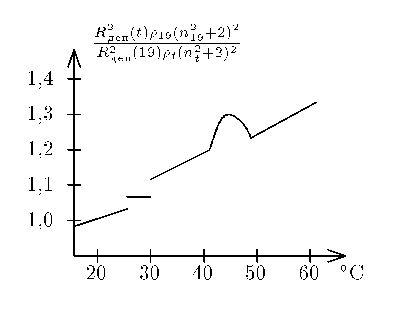
\includegraphics[scale=1]{Ris/ris_eps/ris4_4_08_2.eps}}}

\risp{9}{Температурная зависимость интегральной интенсивности в бензоле}
\end{figure}

Молекулярная структура жидкого безнола была описана с помощью RISM-модели (характеристические взаимодействия узлов с учетом длины межатомных расстояний в молекуле).
Радиальная функция распределения для центров масс $g_{mm}(r)$, центров взаимодействия $g_{ss}(r)$ и центров масс---центров взаимодействия $g_{ms}(r)$ были расчитаны методом Монте-Карло.
Авторы сделали вывод, что в жидком бензоле наряду с характерными для твердого тела взаимноперпендикулярными расположениям молекул могут существовать <<стопочные>> конфигурации.
В расчете RISM-модели было принято во внимание существование постоянного квадрупольного момента в центре бензольного кольца. Центры взаимодействия были выбраны совпадающими с шестью атомами углерода.

Сравнение результатов расчета, полученного методом молекулярной динамики, с результатами экспериментов по рассеянию нейтронов и $x$-лучей показали, что в жидком бензоле может существовать три типа агрегатов, образованных соответствующими димерами:

L-конфигурация, в которой по крайней мере один атом водорода в молекуле, помещенный в начале координат, контактирует
с атомом водорода и атомом углерода соседней молекулы, и пара молекул образует косо касающиеся колеса, чьи оси C$_6$ расположены под прямым углом одна к другой;

стопочная конфигурация --- молекулы распологаются одна над другой, концы колец слегка сдвинуты;

T-конфигурация, в которой атом углерода одной молекулы располагается возле центра другой молекулы, оси C$_6$ соседних
молекул образуют угол, близкий к 90$^{\circ}$.

Возможность одновременного сосуществования различных димеров молекул бензола приводят к образованию локальной структуры
различной симметрии. 
При анализе функции потенциальных взаимодействий для различных моделей взаимной оиентации молекул бензола было показано, что глубины потенциальной ямы различались:

для T-конфигурации $ U_{min}= -8,5$ кДж/моль;

для L-конфигурации $ U_{min}= -6$ кДж/моль;

для стопочной конфигурации $ U_{min}= -4$ кДж/моль.

Различие очень мало, следовательно, если температура жидкости изменяется, можно ожидать сильное изменение между долями,
принадлежащими различным конфигурациям димеров, и, следовательно, изменение симметрии соответствующих локальных структур.

Такое перераспределение приводит к изменению параметра $g_2$, являющегося самымы важным параметром, описывающим структуру молекулярных жидкостей.
Можно показать, что $g_2$ может быть выражено через фурье-преобразование полной корреляционной функции site--site RISM модели, принимая во внимание длины межатомных связей. Для аксиально-симметричных молекул, как мы видели выше,

$$g_2=1+\left<{1\over2}\sum\limits_{k\not= L}(3cos^2\Theta_{KL}-1)\right>, \noq$$
где $\Theta_{KL}$~--- угол между осями симметрии молекул $K$ и $L$.

Значение $g_2=1$ соответствуюет или полному отсутствию ориентационной корреляции, или взаимной компенсации между различными
количествами параллельно ($g_2>1$) и перпендикулярно ($g_2<1$) ориентированных молекулярных димеров.
Можно сделать вывод, что именно $g_2$ является свидетельством изменения в распределении долей локальных структур различной симетрии.

Вернемся к рис. 4.4.9. Условия эксперимента требовали, чтобы кювета с образцом выдерживалась при каждой температуре не менее 3 часов перед началом измерений. Если это не делалось, то в местах изменения наклона кривой $I_h^v(T)$, а также
в местах максимума и минимума результаты не ложились на кривую, наблюдалось <<облако>> точек, в то время как при других температурах точки ложились на кривую без предварительного термостатирования.

Близость $U_{min}\sim kT$ требует большого времени для достижения нового равновесия между долями различных локальных структур, и, следовательно, установления конфигурации с другой локальной симметрией.
Как было показано в работе Рождественской и Эйднера, если разности энергии для различных взаимных расположений молекул бензола
мала, необходимо длительное время, в течение которого система проходит всевозможные состояния, пока не попадет в состояние с $U_{min}$, соответствующей T, L или <<стопочной>> конфигурации в локальной структуре. Незначительные приросты $\Delta Q$ при нагревании приводят систему в состояние с более глубоким значением $U_{min}$ для взаимного расположения молекул в локальной структуре (T к L, L к <<стопке>>).
Для бензола при низкой температуре $g_2<1$. В тройной точке $g_2\sim\hbox{0,7}$, преобладание T-димеров, характерных для состояния твердого тела.

Однако расчеты по методу Монте-Карло показали, что вблизи тройной точки в функции распределения центра масс $g_{mm}(r)$ появляются <<малые>> плечи около 4А, соответствующие димеру стопочной конфигурации. При дальнейшем росте температуры
возрастает количество стопочных и L-димеров. Возможно, что в области, где наклон резко возрастает, увеличивается доля
структур, чья симметрия определяется параллельными стопочными конфигурациями.

Далее при более высоких температурах наблюдается непрерывный рост кривой, отражающий $\gamma_{\hbox{\ris эфф.}}^2\rightarrow \gamma^2_{\hbox{\ris газ}}$ (для бензола $\gamma^2_{\hbox{\ris эфф.}}=24$ и $\gamma^2_{\hbox{\ris газ}}=34/36$).

\vskip 3 mm
\noindent{\bfseries Литература:}
\vskip 1mm
1. {\itshape Флайгер У.} Строение и динамика молекул. --- М.: Изд-во Мир, 1982.

2. {\itshape Рождественская Н. Б., Смирнова Л. В.} Письма в ЖЭТФ, 44, 165. 1982.


3. {\itshape Rozhdestvenskaya N. B., Smirnova L. V., }J. Chem. Phys. 195,
1223.(1991).


4. {\itshape Рождественская Н. Б., Эйднер К.} Вестник ЛГУ (физика химии), 10, 50. 1978.

5. {\itshape Rozhdestvenskaya N. B. and Gorbachova E. N.,
}Optics Commun.
30, 383 (1979).



